\documentclass[UTF8, 11pt, a4paper]{ctexart}
\usepackage{geometry}                		% See geometry.pdf to learn the layout options. There are lots.
\geometry{a4paper} 
%\geometry{landscape}                		% Activate for rotated page geometry
%\usepackage[parfill]{parskip}    		% Activate to begin paragraphs with an empty line rather than an indent
\usepackage{graphicx}				% Use pdf, png, jpg, or eps§ with pdflatex; use eps in DVI mode
								% TeX will automatically convert eps --> pdf in pdflatex		
\usepackage{amssymb}
%% LaTeX - Article customise

%%% PACKAGES
\usepackage{booktabs} % for much better looking tables
\usepackage{array} % for better arrays (eg matrices) in maths
\usepackage{paralist} % very flexible & customisable lists (eg. enumerate/itemize, etc.)
\usepackage{verbatim} % adds environment for commenting out blocks of text & for better verbatim
\usepackage{subfigure} % make it possible to include more than one captioned figure/table in a single float
% These packages are all incorporated in the memoir class to one degree or another...

%%% ToC APPEARANCE


\usepackage{graphicx,amssymb}
\usepackage{fontspec,xltxtra,xunicode}
\usepackage{caption,float,hyperref}
\usepackage{amsmath, amssymb}

%% END Article customise
%SetFonts
%\setCJKmainfont[BoldFont=Songti SC Bold, ItalicFont=Songti SC]{Songti SC}
%\setCJKsansfont[BoldFont=Songti SC Bold]{Songti SC}
%\setCJKmonofont{Songti SC}

\setmainfont{Times New Roman}
\defaultfontfeatures{Mapping=tex-text}
\setromanfont[Mapping=tex-text]{Times New Roman}
\setsansfont[Scale=MatchLowercase,Mapping=tex-text]{Times New Roman}
\setmonofont[Scale=MatchLowercase]{Times New Roman}

%SetFonts
\hbadness=10000
\tolerance=10000
\hfuzz=150pt

\title{A Very Brief Glimps On Complex Networks}
\author{陈思宇\texttt{sychen@zju.edu.cn}}
\date{\today}  


\begin{document}
\maketitle

\begin{abstract}
This article introduces the concepts, methods, and some newest research of complex networks. Since the area of complex networks covers massive contents and topics, in this article, we only promise the delivery of a very short yet brief glimps on Complex Networks.
\end{abstract}

\newpage
\tableofcontents
\newpage


\section{Why complex networks?}

The disscussion about complex networks often comes to the description and definition of it. However, respecting the fact that the definition of complex networks is pretty general, we shall firstly take a look at some concepts.

\begin{itemize}
\item Community evolution
\item Overlapping communities
\item Directed networks
\item Community characterization\ interpretation
\item Modularities
\end{itemize}

Of course, those are all bullshits and very hard to understand neither separately nor integerally.

Because of the complexity of network structure and representation, like the relationship between human beings, the description of networks' characteristics are made from a great deal of aspects. That partially explains why there are so many annoying sophisticated concepts.

While the massive concepts obscure the fundaments of complex networks, we can always find it's true nature through it's purpose. On end, the purposes explain the methologies.

The purposes of complex networks research is mainly focused on the following two aspects.

\begin{itemize}
\item Finding unifying principles.
\item Exploring the dynamics.
\end{itemize}


\section{Is complext-networks' research useful?}
Yes, it is useful in our daliy life. For example, like the following applications.
\begin{itemize}
\item finding prevailing products
and set promoting policy / strategies. 
\item finding key users. key users are those who have considerable influence over other users on purchase decisions.
\item pinpointing hot topics and delivering ads.
\item investigating social networks' following relationships to provide sensible search sortings.
\item clustering genes in biological research, to find the closeness-relations between different gene serials and RNA clips in regard of their functionality and structure similarity.
\end{itemize}


\section{What is Complex Networks?}

As mentioned before, the definition of Complex networks is hard to properly summerized. But, extracting those most essential elements, we can refer to the definition given by QIAN Xue Sen.

\begin{itemize}
\item self-organizing
\item sefl-similar
\item attractor (simple,singular)
\item scale-free (power-law)
\item small-world
\end{itemize}

Self-organizing describes the empirical phenomenon that complex structures are actually generated by individuals with various characteristics.

Self similarity means fractal property, as the picture shown below: The top level view of the networks is similar to any sub-view into it's arbitrary branch.
\begin{figure}[H]
	\centering
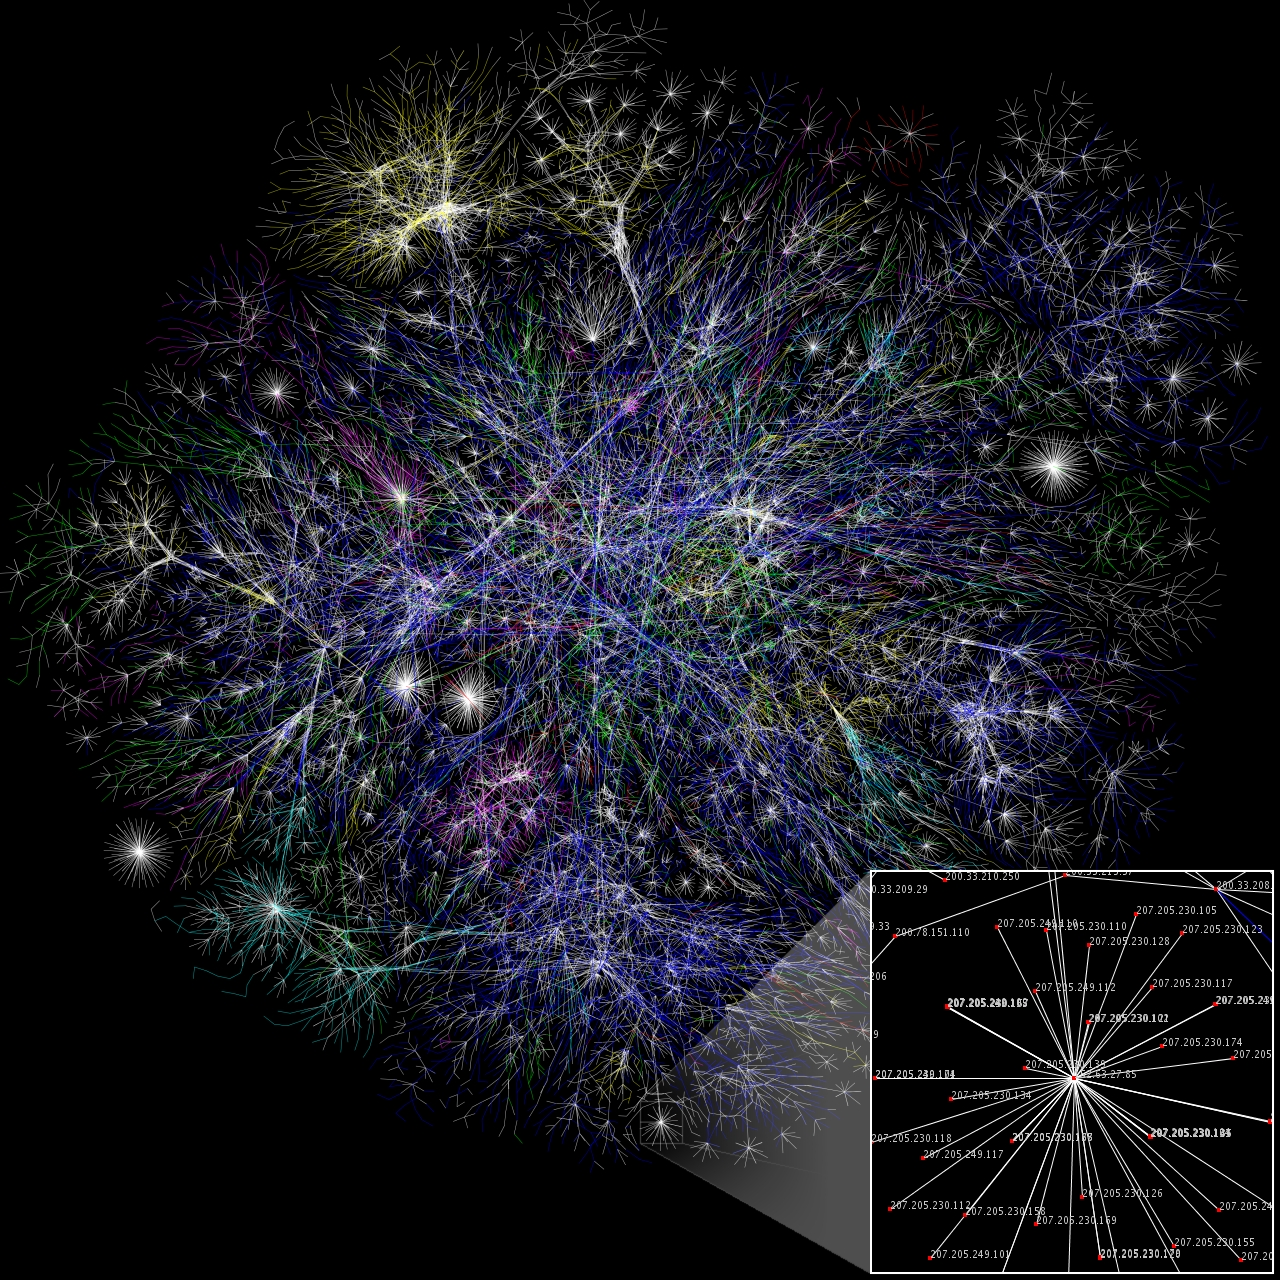
\includegraphics[width=0.80\textwidth]{complexnet}
\caption{}
\end{figure}
Attractor is a state of converge of some complex system. If the state of the system converges to some stable ones, then those states are called simple-attractor. In the opposite case, they are called singular-attractors.

Scale-free is also refered as Power or Long-tail principle, which comes from the statistics of english words' frequency.
\begin{figure}[H]
	\centering
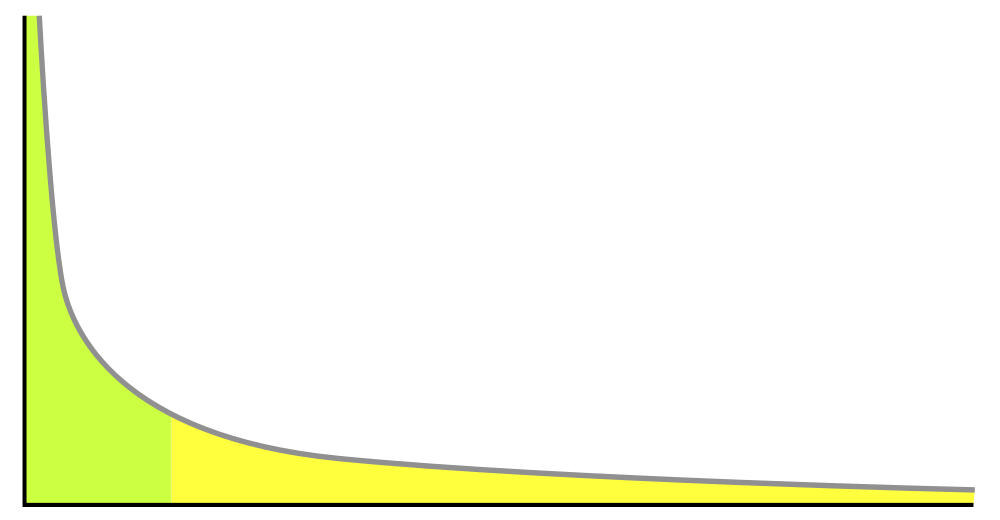
\includegraphics[width=0.80\textwidth]{powerlaw}
\caption{}
\end{figure}
From the chart we see that the probability of a word being preferntially used is of inverse exponential relationship to it's frequency of appearance. This is called Long-tail 
phenomenon.

Later, the concepts purposed like Degree, Closeness($\infty$), and Harmonic Centrality all show explicit Power-law characteristics.

Small-world property demonstrates that the any individual in a complex network tend to have relatively short paths that connect to anyone else. 

Here we shall mention the small world experiment carried out by Milgram in 1967. He randomly send letters to others in another city requesting them to find a way to send those letters back to them as the graph shown below.

\begin{figure}[H]
	\centering
	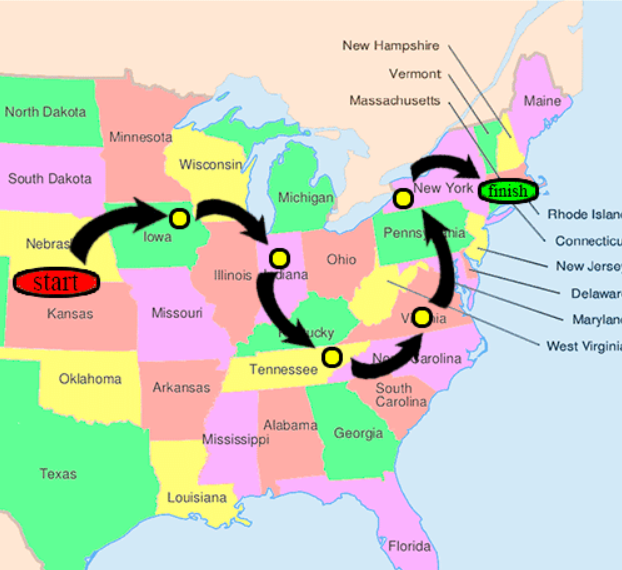
\includegraphics[width=0.80\textwidth]{smallworld}
	\caption{}
\end{figure}

The results are,

\begin{itemize}
\item 232 letters in 296 are lost.
\item 64 letters are returned.
\item average hops is between 5.5 and 6.
\end{itemize}

\section{Some Characteristics}

\begin{itemize}
\item Assortative Mixing: 
$E(i,j), \Delta(node_i,node_j)$ is small.
\item Density $\frac{\text{avg deg}}{\text{complete deg}}$ smells cluster.
\item Pearson corl-coeff:
$cov(x,y)=E[(x-E[x])(y-E[y])], \frac{cov(x,y)}{\sigma_x \sigma_y}$
\item Scalar attributes tends to be correlated.
\item Probablistic properties: 
hidden vars behined time span.(Gaming)
\end{itemize}


Different complex networks own different properties. Some networks have intrinsic aggregations while some networks don't.

\begin{figure}[H]
	\centering
	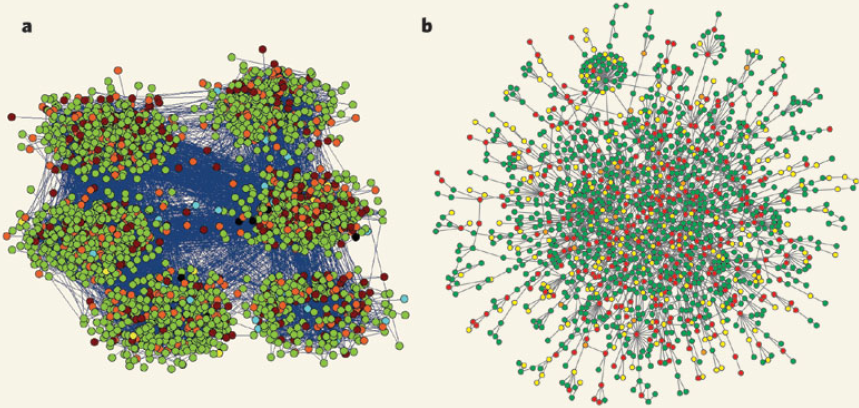
\includegraphics[width=0.80\textwidth]{assort_disassort}
	\caption{}
	a: school communities; b: proteins in brewer's yeast.
\end{figure}

Now we can know clearly and easily about the following concepts.

\begin{itemize}
\item Clique, which is indeed complete subgraphs.
\item Density, which is defined as $\frac{\text{avg deg}}{\text{complete deg}}$
\item Modularity: used to describe the extent of module-divided formation of networks.
Defined as: measurement of extra edges aside of random connection.
\end{itemize}



\section{Algorithms}

Algorithms concerning about complex networks can be classified as four classes.

\begin{itemize}
\item Heirachical
\item Information theory
\item Graph theory
\item Other stupid fantacies
\end{itemize}

Nevertheless, the algorithms are not restricted to any one specific class nor type. Instead, they are often combined methods involving many different ideas.

\subsection{Erdos-Renyi probability based graph model}

Erdos-Renyi probability based graph model was proposed in 1959. The key idea of this algorithm can be stated as `It is with a probability are any two nodes linked'.

Based on this probablistic view, the existence and creation-process of edges, degrees, clusters and communities can be systematically explained.

($m$ is the number of edges, $k$ is degree)
 
\begin{itemize}
\item $Pr(m)=\binom{\binom{n}{2}}{m} p^m (1-p)^{\binom{n}{2}-m}$
\item $\mathbb{E}[m]=\binom{n}{2}p,\mathbb{E}[k]=\frac{2}{n}\binom{n}{2}p$
\item $Pr(k)=\binom{n-1}{k}p^k(1-p)^{(n-1-k)}$

$Pr(k)\simeq \frac{c^k}{k!}e^c$ (Poisson)
\end{itemize}

Under Erdos-Renyi's assumption, the Phase-transition between ``having at least on big community'' and ``having no community'' can be explained and resolve to the edge-linking probability.
($S$ represents the proportion of the entire networs' nodes that are in the big community)
\begin{itemize}
\item $Pr(\neg e_{i,j})=1-p$
\item $Pr(e_{i,j} \land \neg e_{j,compo})=pu$
\item $u=(1-p+pu)^{n-1}=[1-\frac{c(1-u)}{n-1}]^{n-1}$
\item $\lim_{n \rightarrow \infty} u = e^{-c(1-u)}$, $Pr(e_{i,comp})=1-u=S$
\item $\lim_{n \rightarrow \infty} S = 1-e^{-cS}$
\end{itemize}

We can know that for this network to have a big community, c should at least be bigger than or equal to 1.

\subsection{Girvan - Newman algorithm}
Girvan - Newman algorithm was proposed in 2004. This algorithm is sometimes wrongly called NG.

Some preceding concepts:
\begin{itemize}
\item Vertex bewteeneess: The number of shortest path linking any two nodes which go through this vertex.
\item Edge betweenness: as-is above.
\item Pareto principle: 80/20 rule: 20\% of the nodes owns 80\% of the total degrees.
\end{itemize}

GN algorithm is a breadth first heirachical method.
\begin{figure}[H]
	\centering
	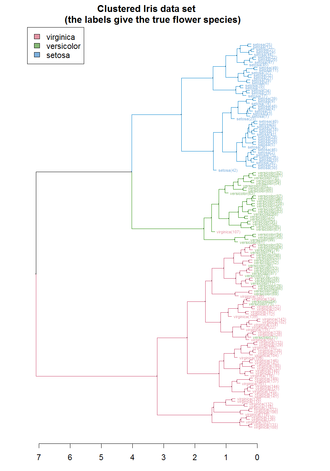
\includegraphics[width=0.50\textwidth]{dendrogram}
	\caption{}
\end{figure}

It continuously remove the edge with highest edge-betweeness to bi-partition the network.

\subsection{Latent Semantic Analysis}
Latent Semantic Analysis was proposed in 1988. This is a method to analyze the semantic classifications of words and sentences.

($D$ means documents, $W$ words, $Z$ topics)
\begin{eqnarray}
D=\{d_1,d_2,..,d_{N} \} \\
W=\{w_1,w_2,..,w_{M} \} \\
Z=\{ z_1,z_2,..,z_{K} \}  \\
A_{coappearance} \text{ is }  N \times M \\
A=U_{N \times r } \Sigma_{r \times r} V^{T}_{r \times M } \text{ (SVD/NMF) }
\end{eqnarray}
$Z$ can be found by applying SVD or NMF technique.


\subsection{Probablistic Latent Semantic Analysis}
Probablistic Latent Semantic Analysis was proposed in 2000 by Thomas Hofmann.
The idea is similar to LSA, but EM is used to determine best topic mappings.
\begin{eqnarray}
P(d_i,w_j)& =& P(d_i) P(w_j | d_i), \\
P(w_j | d_i) &=& \sum_{k=1}^{K} P(w_j | z_k) P(z_k | d_i) \\
\mathcal{L} &=& \sum_{i=1}^N \sum_{j=1}^M n(d_i,w_j) \log P(d_i,w_i)
\end{eqnarray}
EM is dedicated to find best conditional probabiliy about $z$ topics.
\begin{eqnarray}
{\color{red} P(z_k|d_i,w_j) } = \frac{P(z_k)P(d_i|z_k)P(w_j|z_k)}{P(d_i,w_j)} \\
\text{E}[\mathcal{L}] =  \sum_{i=1}^N \sum_{j=1}^M n(d_i,w_j) \sum_{k=1}^{K} \cdot \cdot \cdot  \\
{\color{red} P(z_k|d_i,w_j) } \log  P(w_j|z_k)P(z_k|d_i)
\end{eqnarray}

But, in order to make things clear, we should take a look back on the EM-method.
Furthermore, if we want to know EM better, Lagrange's duality transformation is not to be passed. Hence, we will briefly take a recall on dual problems first.

\subsection{Dual Problem} 
Dual problem is aimed to transform inequity-constrained maximization problem to an equity-constrained minimization one.

\begin{itemize}
\item $f(x), s.t. g(x) \le 0$
\item $L(x,\lambda) = f(x) + \lambda g(x), \lambda \geq 0$
\item $argmax_\lambda L = f =$ initial problem
\item we define original problem as :

$argmin_x argmax_\lambda L(x,\lambda) s.t. \lambda \geq 0, g(x) \leq 0$

\item $ L(x^*,\lambda) \leq L(x^*,\lambda^*)  \leq L(x,\lambda^*)$
\item Karush-Kuhn-Tucker conditions
\end{itemize}
To obtain the best solution, KKT conditions are deduced.
\begin{itemize}
\item $\lambda^* g(x^*)=0$
\item $\frac{\partial L}{  \partial x} =0$ 
\item $\lambda \geq 0 , g(x) \leq 0$
\end{itemize}
KKT is necessary and sufficient condition.
\begin{itemize}
\item $\max_\lambda \min_x L(x,\lambda) , s.t. \lambda \geq 0, g(x) \leq 0$
\item KKT $\rightarrow x=h(\lambda)$
\item $\max_\lambda L(h(\lambda),\lambda) s.t. \lambda \geq 0, S(\lambda)=0$
\end{itemize}


\subsection{Expectation Maximization}
Having recalled dual problems, now we take a short tour through Expectation Maximization.
\begin{itemize}
\item $f(x;\theta) \rightarrow f(x,y;\theta)$
\item randomize $\theta, y$
\item estimate $Q=q(y,\theta)$ (E-step)
\item $\frac{\partial -L(Q)}{\partial \theta}=0$,update $\theta$ (M-step)
\item repeat until converge.
\end{itemize}
The convergence is guaranteed by the following deduction.
\begin{itemize}
\item Jensen's inequality $f(\sum \lambda x) \leq \sum \lambda f(x)$
\item $\sum \log \sum p \geq \sum \sum Q \log \frac{p}{Q}=l(\theta) $
\item $l(\theta)$ is the lower bound. 
\item $f(E_z[\frac{p(x,z;\theta)}{Q(z)}]) \geq E_z[f(\frac{p(x,z;\theta)}{Q(z)})]$
\item $\frac{p}{Q}=Const$ s.t. $\sum_z Q(z)=1$
\item $Q(z)=\frac{p(x,z)}{\sum p(x)}=p(z|x;\theta)$
\end{itemize}

Now we can happily use EM to perform optimization solvings.

\subsection{Ball,Karrer,Newman algorithm}
Ball,Karrer,Newman algorithm is called BKN for short, and is able to detect overlappings.
\begin{figure}[H]
	\centering
	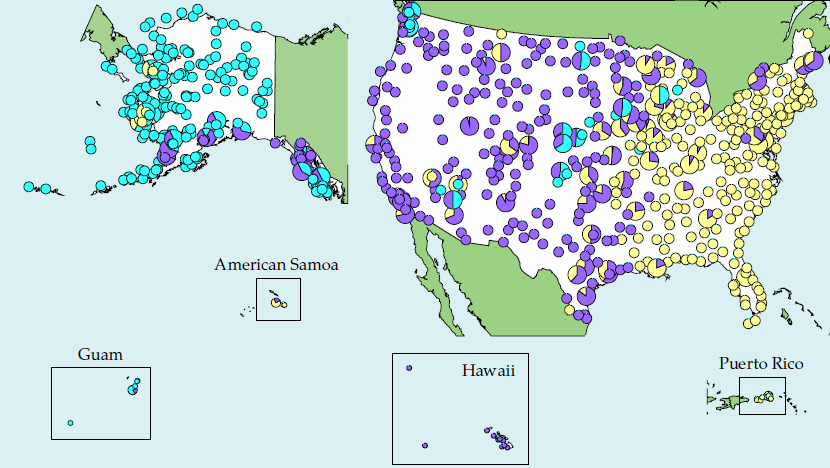
\includegraphics[width=0.80\textwidth]{bkn}
	\caption{}
\end{figure}
the figure

\subsection{Latent community discovery network}
\begin{itemize}
\item how to get a list of core actors?
\item $\sum_z P(z|d)=1$,(mixing) 
\item $\sum_a P(a|z)=1$ (topics are prevailing)
\item $L=\sum_d \sum_a C(a,d) \log \sum_z P(a|z)P(z|d)$
\item $R=\sum_{a1,a2} \sum_z \|p(z|a_1) - p(z|a_2)\|^2$ what?
\end{itemize}
Problem definition and solving.
\begin{itemize}
\item $Objective=\alpha (-L) + (1-\alpha)R$
\item EM again.
\end{itemize}
Results on DBLP co-authorship.
(AI DB DP GV NC)
\begin{figure}[H]
	\centering
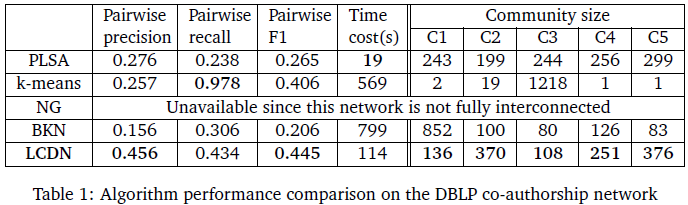
\includegraphics[height=3.5cm]{lcdndblp}
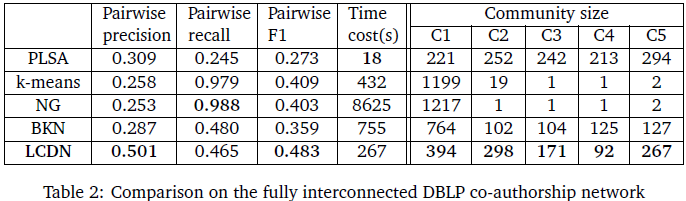
\includegraphics[height=3.5cm]{lcdndblpfully}
	\caption{}
\end{figure}
Then the experiment was carried out on WEIBO network.
1. Entertainment244 2. Leisure,  333 
3. Finance,  297 4. Culture,  185
5. Media,  163 
\begin{figure}[H]
	\centering
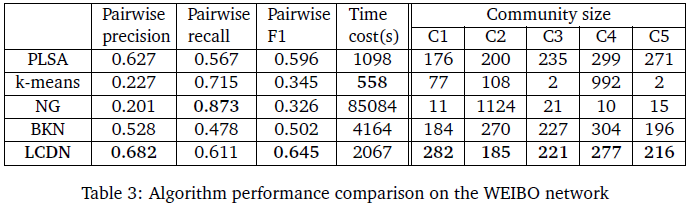
\includegraphics[height=3.5cm]{lcdnweibo}
	\caption{}
\end{figure}
The results is pretty good. However we should notice that, if you torture the data long enough, data will confess.



\subsection{Page rank}
Page rank was firstly applied in 1998. The algorithm is a fairly simple one but really works.
\begin{itemize}
\item incoming-links: other $\rightarrow$ this site.
\item Pagerank(site) $PR(site)$
\item $PR(A)=\left( \frac{PR(B)}{L(B)} + \frac{PR(C)}{L(C)} + \cdots \right)d + \frac{1-d}{N}$
\item $(1-d)$
\end{itemize}
Later, some page-rank-like algorithms were also proposed like:
\begin{itemize}
\item Idealrank 2009: local pagerank. far-away PR-values are simplified and unified.
\item $\lim_{\substack{edge \rightarrow full \\ V_{local} \rightarrow V_{global} } } Idealrank= Pagerank$
\item approxrank 2009:  $approxrank \sim Idealrank$
\end{itemize}

\subsection{Trust Network}
Trust networks are related to the topics listed below.
\begin{itemize}
\item e-commerce
\item resource sharing
\item SQA,SDN
\item propagenda
\item promotion/ads
\end{itemize}

An algorithm on trust network was proposed by Zhang shaozhong. et al.  2012
\begin{itemize}
\item Interactions matrix $A$
\item Successful Interactions matrix $T$
\item Faliures $F$
\item $Believe(v_i,v_j)=\sum \sum p(v_i,v_j) \log \frac{p(v_i,v_j)}{p(v_i)p(v_j)} $
\item $v$: success or failure.
\end{itemize}

this method use Mutual information as basic metric.

$I(X;Y) = \sum_y \sum_x  p(x,y) \log \frac{p(x,y)}{p(x)p(y)} $

if $X, Y$, iid. then $ I=0$

else $ I > 0 $

To find an optimal trusty path, we can apply the following ways.
\begin{itemize}
\item Floyd
\item Dijkstra
\end{itemize}
But the further question is how to find communities?
Zhang gave a way by minimizing total edge number while maximizing connectivity.  
\begin{itemize}
\item interconnectivity in v $C_v = \frac{2t_v}{k_v(k_v-1)} $
\item $\text{E}[C_v]=C=\frac{\sum_{n=1}^{\infty} C_v}{n} $
\item characteristic path length: $\frac{\sum_i \frac{\sum_j MinDist(i,j)}{n-1}  }{n} $
\end{itemize}
The setps are like followings.
\begin{itemize}
\item $ f = a \left( \sum Believe \right) + b C|_m $
\item cut $m$ weak interactions. (heirachical?)
\item {\color{red} NP hard!}
\item a heuristic algorithm:
 \item [1] cut $m$ edges $e_1,..,e_m$ that maximize $f$.
 \item [2]  add $e_m'$ that maximize $f$, if $e_m' =e_m$ over.
 \item [3] cut one edge that maximize $f$, then go to 2.
\end{itemize}

\end{document}
